\documentclass[journal=jpcafh]{achemso}

\usepackage{booktabs}
\usepackage{paralist}
\usepackage{nicefrac}
\usepackage{hyperref}
\usepackage{rotating}

\usepackage{subcaption}
\newcounter{subscheme}
\renewcommand{\thesubfigure}{\alph{subfigure}}
\renewcommand{\thesubscheme}{\thescheme\alph{subscheme}}

\usepackage{siunitx}
\DeclareSIUnit \au{a.u.}

\usepackage[version=3]{mhchem}
\usepackage{braket}

%% TIKZ
\usepackage{tikz}

\allowdisplaybreaks

\title{Influence of symmetry and electronic structure parameters on NLO properties: insights from the few state approximation}
\date{Version of \today}
\author{Pierre Beaujean}
\author{Benoît Champagne}
\email{benoit.champagne@unamur.be}
\affiliation{Laboratory of Theoretical Chemistry, 
	Unit of Theoretical and Structural Physical Chemistry, 
	Namur Institute of Structured Matter, 
	University of Namur, 
	Rue de Bruxelles 61, B-5000 Namur, Belgium}

\begin{document}
\maketitle

\begin{abstract}
	TO BE CONTINUED
\end{abstract}

\section{Introduction}

In nonlinear optics (NLO), promising molecular architectures often belong to the push-pull family. These structures typically consist of electron donor and acceptor groups connected by a $\pi$-conjugated segment that facilitates electronic ``communication'' between the two moieties.

To elucidate the relationships between NLO properties and structure, simplified models have been developed to capture complex phenomena with minimal parameters. The valence-bond charge-transfer (VB-CT) model, pioneered by Mulliken \cite{mullikenMolecularCompoundsTheir1952}, has been particularly successful in describing the first hyperpolarizabilities of push-pull polyenes. It also applies to other properties, such as UV/VIS absorption spectra and various physico-chemical characteristics \cite{benderTheoreticalModelsChargetransfer1986}. This model represents a system as a superposition of two limiting states, a valence-bond state, $\phi_{VB}$, and a charge-transfer state, $\phi_{CT}$, connected by electron displacement from the donor to the acceptor (Scheme \ref{sc:vbct}). Using fundamental parameters, such as the ionization energy of the donor, electron affinity of the acceptor, and the coupling between these states, the VB-CT model provides valuable insight into structure-activity relationships.  Indeed, when combined with the sum-over-states (SOS) theory developed by Orr and Ward \cite{orrPerturbationTheoryNonlinear1971}, these models provide estimate of NLO properties and identification of valuable structure-activity relationships.


\begin{scheme}[!h]
	\centering
	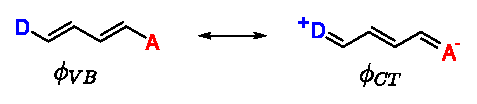
\includegraphics[width=.5\linewidth]{Scheme1}
	\caption{Limiting forms of the VB-CT model.}
	\label{sc:vbct}
\end{scheme}

Despite its simplicity, this model has proven versatile, allowing extensions to systems with multiple donor/acceptor groups through 3-state \cite{hahnNonlinearOpticalProperties1999,barzoukasMolecularEngineeringPush2000,yangLargeOffDiagonalContribution2003}, 4-state \cite{choElementaryDescriptionNonlinear1998}, and 5-state \cite{choNonlinearOpticalProperties2002} descriptions. 
Further generalization are also possible\cite{alamGeneralizedFewstateModel2020} in order to get deeper understanding of the NLO responses, although at the cost of an increasingly large number of parameters.
However, to the best of our knowledge, a comparison of the performances of these different model has not been attempted. Therefore, this paper aims at providing a comparative analysis of the  VB-$n$CT models with $n$=1-4  (Scheme \ref{sc:vbct}) .  To provide further insights, this analysis is performed  using the experimental quantities found using the second harmonic scattering measurement technique.\cite{verbiestSecondOrderNonlinearOptical2009}
It is organized as following: after a brief reminder of the different formulations of the VB-$n$CT models, of the relevant quantities, and of the different models, the main results are compared. Finally, the last section draws conclusions and perspectives.

\begin{scheme}
	\caption{Simplified representation of the successive VB-$n$CT models ($n\in[1,4]$, adapted from Cho \latin{et al.}\cite{choNonlinearOpticalProperties2002}, with the charge transfer integrals $t$ and $T$). Donor (D, in blue) and acceptor (A, in red) can be swapped without loss of generality.}
	\label{sc:mct}
	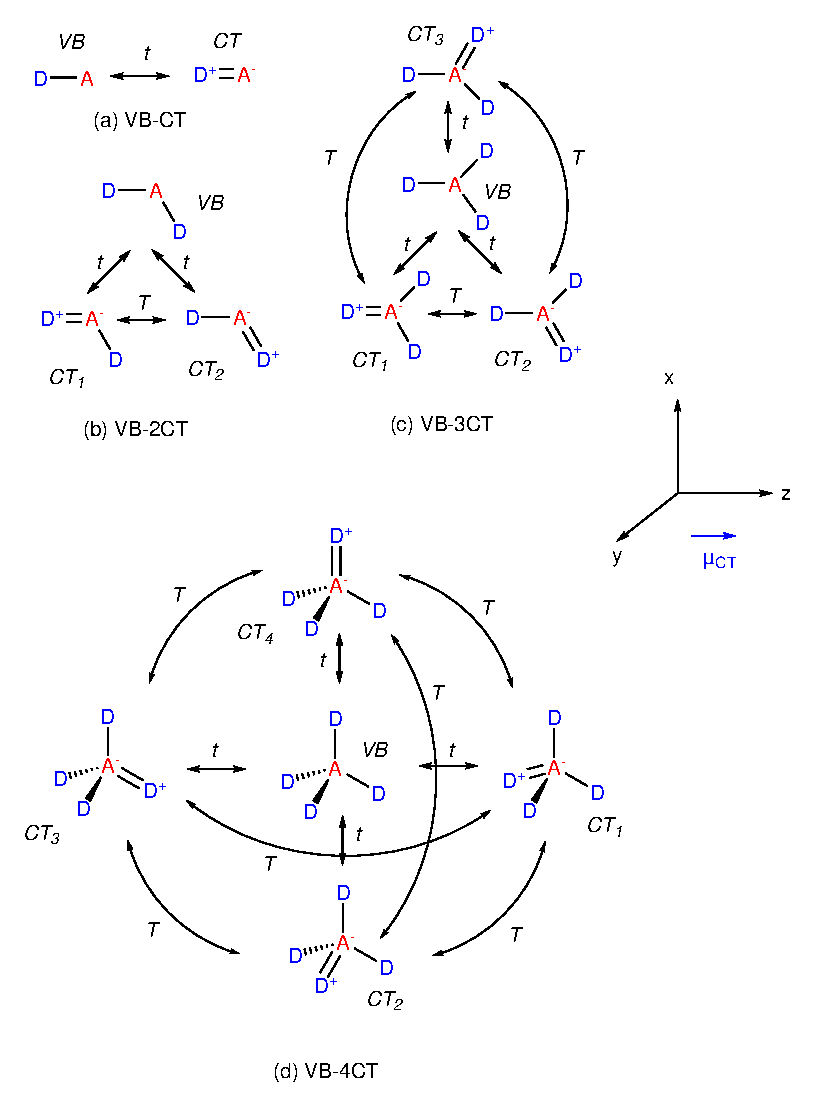
\includegraphics[width=.5\linewidth]{Scheme2}
\end{scheme}



\section{Theory \label{sec:theory}}

\subsection{A model Hamiltonian for the VB-$n$CT model}

Using the variational approach, given a set of basis functions $\{\phi_i\}$, the energy of a trial function $\Psi = \sum_i c_i \phi_i$ is always greater than or equal to the true ground state energy, $\varepsilon_0$:\begin{equation}
	\mathcal E_0 \leq 	\mathcal E, \text{ where }	\mathcal E = \frac{\braket{\Psi|H|\Psi}}{\braket{\Psi|\Psi}}, \label{eq:variational}
\end{equation}
One minimizes the energy of the trial function by setting $\frac{d	\mathcal E}{dc_i} = 0$. 
This yields a set of so-called secular equations of the form:\begin{equation}
	\forall k: \sum_i c_i (H_{ki} - \varepsilon_k S_{ki}) = 0, 
\end{equation}
where $S_{ki} = \braket{\phi_k | \phi_i}$ (overlap matrix) and $H_{ki} = \braket{\phi_k | \hat{H} | \phi_i}$ (Hamiltonian matrix). 
This is a generalized eigenvalue problem. 
If the basis functions are orthogonal, i.e., $S_{ki} = \delta_{k,i}$, this reduces to a standard eigenvalue problem, $HC=C\varepsilon$, where diagonalizing $H$ gives the energy levels, $\{\varepsilon_k \}$. $C$ is the matrix of coefficients, also referred to as the eigenfunctions of the system.

In the VB-$n$CT framework, corresponding to a $(n+1)$-state model, a set of orthogonal functions is employed consisting of one valence-bond (VB) state, $\phi_{VB}$, and $n$ charge-transfer (CT) states, $\{\phi_{CT,i}|0<i\leq n\}$. This leads to a model Hamiltonian, given by a $(n+1)\times(n+1)$ matrix and parameterized as follows:
\begin{align}
	&\braket{\phi_{VB}|\hat{H}|\phi_{VB}} = E_{VB}, 
	\braket{\phi_{VB}|\hat{H}|\phi_{CT,i}} = -t, \text{ and } 
	\braket{\phi_{CT,i}|\hat{H}|\phi_{CT,j}} = \begin{cases}
		E_{CT} & \text{if } i=j,\\
		-T & \text{otherwise},
	\end{cases}\label{eq:hamilonian}
\end{align}
where $E_{VB}$ and $E_{CT}$ denote the energies of the VB and CT states, respectively, while $t$ and $T$ are the transfer integrals. 

Solving the eigenvalue problem yields a ground state, $\ket{0}$, with minimal energy, a set of $(n-1)$-fold degenerate excited states, $\{\ket{e_i} | 0<i< n\}$ (which does not exists when $n=1$), and a single non-degenerate excited state, $\ket{f}$.
Corresponding eigenvalues were provided by Cho \emph{et al.} \cite{choNonlinearOpticalProperties2002} and are, in all generality, given by:
\begin{align}
	E_{0} &= \frac{1}{2} \left[E_{VB} + E_{CT} - (n-1)T - \sqrt{(V - (n-1)T)^2 + 4nt^2}\right], \nonumber\\
	E_{e_i} &= E_{CT} + T, \nonumber\\
	E_{f} &= \frac{1}{2} \left[E_{VB} + E_{CT} - (n-1)T + \sqrt{(V - (n-1)T)^2 + 4nt^2}\right],
\end{align}
where $V = E_{CT} - E_{VB}$. 
The associated eigenfunctions are:
\begin{align}
	\ket{0} &= \cos\delta\,\ket{\phi_{VB}} + \frac{\sin\delta}{\sqrt{n}} \sum_{0<j\leq n} \ket{\phi_{CT,j}},\nonumber\\
	\ket{e_i} &= \frac{1}{\sqrt{i(i+1)}}\left[- \sum_{0<j\leq i} \ket{\phi_{CT,j}} +  i \ket{\phi_{CT,i+1}}\right],\nonumber\\
	\ket{f} &= \sin\delta\,\ket{\phi_{VB}} - \frac{\cos\delta}{\sqrt{n}} \sum_{0<j\leq n} \ket{\phi_{CT,j}},
\end{align}
where the mixing angle $\delta \in [0, \nicefrac{\pi}{2}]$ is introduced. For $0 \leq \delta < \nicefrac{\pi}{4}$, the ground state is VB-dominated, whereas for $\nicefrac{\pi}{4} < \delta \leq \nicefrac{\pi}{2}$, the CT state dominates. The point $\delta = \nicefrac{\pi}{4}$ is referred to as the \textit{cyanine limit}.

Minimizing the ground-state energy $E_0$ with respect to $\delta$ (see Eq.~\eqref{eq:variational})  provides a condition linking the parameters:
\begin{equation}
	\frac{\partial E_0(\delta)}{\partial \delta} = 0 \Rightarrow V - (n-1)T = 2t \sqrt{n} \cot(2\delta). \label{eq:cot}
\end{equation}
Setting the energy origin to:
\begin{equation}
	E_{VB} + E_{CT} - (n-1)T = 0, \label{eq:eorig}
\end{equation}
simplifies the eigenvalues to:
\begin{align}
	E_{0} = -\sqrt{n} \frac{t}{\sin(2\delta)}, E_{e_i} = nT + t \sqrt{n} \cot(2\delta), \text{ and }
	E_{f} =  \frac{t}{\sin(2\delta)}\sqrt{n}.\label{eq:energies}
\end{align}
In the following analysis, difference between the state energies are employed:\begin{align}
	\Delta E_{0e} &= E_{e_i} - E_{0} = nT + t\,\sqrt{n}\,\cot{(2\delta)} + \sqrt{n}\,\frac{t}{\sin{(2\delta)}}  = t\,\sqrt{n}\,\cot(\delta) + nT,\nonumber\\
	\Delta E_{0f} &= E_f - E_0 = \frac{2t\,\sqrt{n}}{\sin(2\delta)}.
\end{align}

To monitor variations in molecular properties, the charge-transfer (CT) character of the ground state, $\ell_{CT}$, can be introduced as follows \cite{choNonlinearOpticalProperties2002,choElementaryDescriptionNonlinear1998,yangLargeOffDiagonalContribution2003}:
\begin{equation}
	\ell_{CT} = \frac{1}{n} \sin^2 \delta.
\end{equation}
With $\delta \in [0, \nicefrac{\pi}{2}]$, $\ell_{CT}$ varies in the range $\ell_{CT} \in [0, \nicefrac{1}{n}]$. A value of $\ell_{CT} = 0$ indicates a ground state fully described by the VB form, while $\ell_{CT} = \nicefrac{1}{n}$ corresponds to a state entirely characterized by CT. 
An additional parameter, introduced by Barzoukas and collaborators \cite{barzoukasTWOFORMDESCRIPTIONPUSHPULL1996,barzoukasTwostateDescriptionHyper1996,blanchard-desceTwoformTwostateAnalysis1998a}, measures the VB-CT mixing:
\begin{equation}
	m_{CT} = -\cos(2\delta) = 2n \ell_{CT} - 1.
\end{equation} 
This parameter, $m_{CT}$, ranges from $-1$ (VB-dominated) to $+1$ (CT-dominated), effectively capturing the balance between VB and CT character in the ground state. In that framework, the eigenvalues become:\begin{align}
E_{0} = -t\,\sqrt{\frac{n}{1-m_{CT}^2}},
E_{e_i} = nT -t\,\sqrt{n}\,\frac{m_{CT}}{\sqrt{1-m_{CT}^2}},
E_{f} = t\,\sqrt{\frac{n}{1-m_{CT}^2}},
\end{align} 
and the excitation energies now read:\begin{align}
	\Delta E_{0e}= nT + t\,\sqrt{n\,\frac{1-m_{CT}}{1+m_{CT}}}, \Delta E_{0f} = 2t\,\sqrt{\frac{n}{1-m_{CT}^2}}. \label{eq:energiesmct}
\end{align}
The evolution of excitation energies as a function of $m_{CT}$ is shown in Fig.~\ref{fig:eexci}. Notably, both $\Delta E_{0e}$ and $\Delta E_{0f}$ diverge to $+\infty$ as $m_{CT} \to -1$. Similarly, $\Delta E_{0f}$ also tends to $+\infty$ when $m_{CT} \to 1$.  
Moreover, $\Delta E_{0e}$ exhibits a minimum at $m_{CT} = 1$, where $\Delta E_{0e} = nT$, while $\Delta E_{0f}$ reaches its minimum at $m_{CT} = 0$, with $\Delta E_{0f} = 2t\sqrt{n}$. Finally, decreasing both $t$ and $T$ lead to a decrease in $\Delta E_{0f}$ and $\Delta E_{0e}$. This will become important in the following sections, since $X^{(n)} \propto \frac{1}{\Delta E^n} \propto \frac{1}{t^n}$ (see below).


\begin{figure}[!h]
	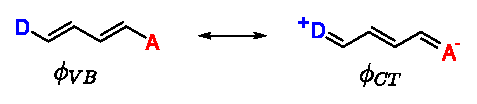
\includegraphics[width=.7\linewidth]{Figure1}
	\caption{Evolution of the reduced $\ket{0}\to\ket{f}$ ($\Delta E_{0f} / t$, unitless, top) and $\ket{0}\to\ket{e}$ ($\Delta E_{0e} /t$, unitless, bottom) excitation energies, computed using $T = t/2$, as a function of the charge transfer character of the ground state ($m_{CT}$).}
	\label{fig:eexci}
\end{figure}

Furthermore, $\ket{0}$ and $\ket{f}$ may be redefined, as:\begin{align}
\ket{0} &= \sqrt{\frac{1-m_{CT}}{2}}\,\ket{\phi_{VB}} + \sqrt{\frac{1+m_{CT}}{2n}}\,\sum_j^n \ket{\phi_{CT,j}},\nonumber\\
\ket{f} &= \sqrt{\frac{1+m_{CT}}{2}}\,\ket{\phi_{VB}} - \sqrt{\frac{1-m_{CT}}{2n}}\,\sum_j^n \ket{\phi_{CT,j}}.
\end{align}

\clearpage

\subsection{Sum-over-state (SOS) expression of NLO tensors}

On the ground of perturbation theory, 
the SOS expression of Orr and Ward \cite{orrPerturbationTheoryNonlinear1971} states that, far from resonance, any component of any nonlinear optical tensor $X^{(n)}(-\omega_\sigma;\omega_1,\ldots)$ (of order $n$, so the polarizability, $\alpha = X^{(1)}$, the first hyperpolarizability $\beta = X^{(2)}$,or the second hyperpolarizability $\gamma = X^{(3)}$) is given by:\begin{align}
	&X^{(n)}_{\zeta\eta\ldots\nu}(-\omega_\sigma;\omega_1,\ldots) = \hbar^{-n}\sum_{\mathcal{P}_F}\sum_{a_1,a_2\ldots\,a_{n}} \frac{\mu^\zeta_{0a_1}{\mu}^\eta_{a_1a_2}\ldots \mu^\nu_{a_{n\,0}}}{\prod_{0<i\leq n} (\omega_{a_i}-\omega_\sigma+\sum_{0<j<i} \omega_j)},\label{eq:sos}
\end{align}
where $\zeta,\eta,\ldots$ are the Cartesian coordinates $x, y, z$ (in the molecular frame), $\omega_1, \omega_2\ldots$, the (optical) input frequencies of the laser for the NLO process (with $\omega_\sigma = \sum_{0<i<n} \omega_i$), $\ket{a_1}, \ket{a_2}, \ldots$, the states of the system  including the ground state (with $\hbar\omega_{a_i}$ the excitation energy from ground state to $\ket{a_i}$), $\mu^\zeta_{a_ia_j} = \braket{a_i|\hat \zeta|a_j}$ the transition dipole moment from state $a_i$ to $a_j$ (it corresponds to the dipole moment of electronic state $a_i$ when $i=j$), and $\sum_{\mathcal{P}_F}$ the sum of all permutations over each pair $(\zeta, \omega_\sigma),(\eta,\omega_1),\ldots$.  However, this expression encounters divergences (or singularities) when a denominator vanishes. In the static case ($\forall i: \omega_i = 0$), it happens when the sum includes the ground state. Following Orr and Ward \cite{orrPerturbationTheoryNonlinear1971} and latter Bishop \cite{bishopExplicitNondivergentFormulas1994}, substituting the dipole operator in Eq.~\eqref{eq:sos} with a fluctuation dipole operator, $\bar{\mu}^\zeta_{a_1 a_2} = \mu^\zeta_{a_1 a_2} - \delta_{a_1 a_2}\, \mu_{00}^\zeta$, results in $\bar{\mu}^\zeta_{00} = 0$, allowing the ground state to be excluded from the summations. Consequently, for the static case, one has:
\begin{align}
	\beta_{(\zeta\eta\kappa)} &=\sum_{\mathcal{P}_F} \sum_{a_1', a_2'} \frac{(\zeta\bar{\eta}\kappa)_{a_1 a_2}}{\Delta E_{0a_1}\,\Delta E_{0a_2}}, \label{eq:sosbeta},
\end{align}
where $\Delta E_{0a_1} = \hbar\omega_{a_1}$, and the prime indicates that the sums over $a_j$ now exclude $\ket{0}$.  Here, the simplified numerator notation of Bishop \cite{bishopExplicitNondivergentFormulas1994}, $(\zeta\eta\kappa)_{a_1 a_2} = \mu_{0 a_1}^\zeta \mu_{a_1 a_2}^\eta \mu_{a_2 0}^\kappa$, is employed. Since this paper focus on the static case, the permutation $\sum_{\mathcal P_F}$ runs over all components, so that $\alpha_{\zeta\eta} = \alpha_{\eta\zeta}$, which is indicated using parentheses, $\alpha_{(\zeta\eta)}$.

To utilize Eq.~\eqref{eq:sosbeta}, both excitation energies, calculated, in the VB-$n$CT model, as differences between eigenvalues, given in Eq.~\eqref{eq:energies} (or, in this contribution, Eq.~\eqref{eq:energiesmct}), and transition/excited-state dipoles are required. In general, these dipoles are computed as follows:
\begin{equation}
\vec{\mu}_{ij} = \braket{i | \hat{\mu} | j} = \sum_{\nu\xi} C_{i \nu} C_{j \xi} \, \braket{\phi_\nu | \hat{\mu} | \phi_\xi} = C\,M\,C^\dagger,
\end{equation}
where $\ket{i} = \sum_\nu C_{i \nu} \, \ket{\phi_\nu}$ represents the electronic states of the system, $C_{i \nu}$ are the coefficients in the state expansion, and $\ket{\phi_\nu}$ are the basis functions. 
In the VB-$n$CT model, the dipole matrix elements $M_{\nu\zeta} = \braket{\phi_\nu | \hat{\mu} | \phi_\zeta}$ are given as follows \cite{luValenceBondChargeTransferModel1994}:
\begin{align}
\braket{\phi_{VB} | \hat{\mu} | \phi_{VB}} = \braket{\phi_{VB} | \hat{\mu} | \phi_{CT,i}} = 0,
\braket{\phi_{CT,i} | \hat{\mu} | \phi_{CT,j}} = 
\begin{cases}
	\vec{\mu}_{CT,i} & \text{if } i = j, \\
	0 & \text{otherwise}.
\end{cases}
\end{align}
This results in a sparse, diagonal dipole matrix parameterized by a select set of CT dipole moments associated to each CT state, $\{\vec{\mu}_{CT,i} \mid 0 < i \leq n\}$. Generally, $\vec\mu_{CT, i} = \mu_{CT}\,\vec{e}_i$, where $\vec  e_i$ is a unit vector, so that all dipole have the same length, given by the quantity $\mu_{CT}$.  

As a result, the ground-state, transition, and excited-state dipole moments are all proportional to $ \mu_{CT}$. Since the excitation energies scale with the parameter $t$, and in light of Eq.~\eqref{eq:sos}, reduced hyperpolarizabilities (denoted with a tilde) are introduced in this work. These dimensionless quantities are defined for any component of the tensors, as:
\begin{equation}
	\tilde\beta = \beta \times \frac{t^2}{\mu_{CT}^3}. \label{eq:reduced}
\end{equation}

 
\subsection{Tensor invariants}

For an isotropic medium composed of identical molecules or scatterers, the intensity, $I^{(n\omega)}$, of the incoherent contribution to the $n$-uple harmonic scattered light is proportional to an isotropic (or rotational) averaging of the tensor elements over all possible molecular orientations, $\braket{X^{(n)}}$ \cite{Andrews1980,verbiest_second-order_2009,Castet2012,fordMolecularTensorAnalysis2018}.
For the second harmonic scattering (SHS), the conventional experimental setup is the hyper-Rayleigh scattering (HRS) technique\cite{verbiestSecondOrderNonlinearOptical2009}, where the scattered light is analyzed at a \SI{90}{\degree} angle with respect to the direction of propagation ($Y$), the fundamental light beam (of frequency $\omega$) is $Z$- or $X$-polarized (in the laboratory frame), while the $Z$-linearly polarized component of the scattered beam (of frequency $2\omega$) is recorded in the $X$ direction. One can thus distinguish between two polarization combinations: the VV geometry (vertical-vertical, both incident and scattered lights are $Z$-polarized) and HV [horizontal-vertical, the incident (scattered) light is $X$ ($Z$)-polarized]. The $I_{VV}$ intensity is proportional to $\braket{\beta_{ZZZ}^2}$, while $I_{HV}$ is proportional to $\braket{\beta_{ZXX}^2}$.
For a non-po\-la\-ri\-zed incident signal, both polarizations have equal probability and the intensity becomes proportional to the sum of the HV and VV observables. This allows defining $\beta_{SHS}$, the average first hyperpolarizability, and a depolarization ratio:\begin{align}
	\beta_{SHS} = \sqrt{\braket{\beta_{ZZZ}^2}+\braket{\beta_{ZXX}^2}} \text{ and } \text{DR}_{SHS} = \frac{\braket{\beta_{ZZZ}^2}}{\braket{\beta_{ZXX}^2}}.\label{eq:bhrs}
\end{align}
Furthermore, the $\beta$ tensor can be decomposed into irreducible spherical components\cite{Jerphagnon1978}. When assuming the Kleinman's conditions (since only the static case is addressed in this article), $\beta$ contains a dipolar ($J$ = 1) and an octupolar ($J$ = 3) component \cite{Brasselet1998}, expressed as:\begin{align}
	&|\beta_{J=1}|^2 = \frac{3}{5}\sum_{\zeta\eta\kappa}^{x,y,z} \beta_{\zeta\eta\eta}\beta_{\zeta\kappa\kappa} \text{ and }|\beta_{J=3}|^2 =\sum_{\zeta\eta\kappa}^{x,y,z} \beta_{\zeta\eta\kappa}^2 - \frac{3}{5} \beta_{\zeta\eta\eta}\beta_{\zeta\kappa\kappa}. \label{eq:bj}
\end{align}
As a consequence:\begin{align}
		\braket{\beta^2_{ZZZ}} =  \frac{1}{5}\,|\beta_{J=1}|^2+\frac{2}{35}\,|\beta_{J=3}|^2 \text{ and } \braket{\beta^2_{ZXX}} = \frac{1}{45}\,|\beta_{J=1}|^2+\frac{4}{105}\,|\beta_{J=3}|^2.\label{eq:beta2}
\end{align}
Notably, it implies that in the octupolar limit (when $|\beta_{J=3}|^2 \gg |\beta_{J=1}|^2$) DR$_{SHS}\to\frac{3}{2}$, which is the minimal value it can take. It reaches a maximal value of $9$ in the dipolar limit.\cite{verbiest_second-order_2009}

Note that as a consequence of Eq.~\eqref{eq:reduced}, one can define $\tilde\beta_{SHS}$ in a similar way.

\subsection{Model systems}

The following model systems are considered in this article. For each of them, the expression for \begin{inparaenum}[i)]
	\item the ground-state, transition, and excited states dipole moments,
	\item the non-null tensor components [obtained using Eq.~\ref{eq:sos}], and
	\item the rotational invariants [obtained using Eq.~\eqref{eq:beta2}]
\end{inparaenum} are reported in the Supporting Information (SI).

\paragraph{Two-state $C_{\infty v}$ systems.}  
This model consists of a single donor-acceptor (D/A) pair, typically positioned at the extremities of a $\pi$-conjugated linker. For convenience, it is oriented along the $z$-axis, such that the charge transfer dipole moment is given by:  
\begin{equation*}
	\vec{\mu}_{CT} = \mu_{CT} \begin{pmatrix} 0 \\ 0 \\ 1 \end{pmatrix}.
\end{equation*}

\paragraph{Three-state $C_{2v}$ systems.}  
This system extends the two-state model by introducing two charge transfer (CT) states with dipole moments forming an angle $\theta \in [0, \nicefrac{\pi}{2}]$ relative to the $z$-axis \cite{yangLargeOffDiagonalContribution2003}, as illustrated in Scheme~\ref{sc:mu}. The dipole moments are thus expressed as:  
\begin{equation*}
	\vec{\mu}_{CT,1} = \mu_{CT} \begin{pmatrix} \sin\theta \\ 0 \\ \cos\theta \end{pmatrix}, \quad  
	\vec{\mu}_{CT,2} = \mu_{CT} \begin{pmatrix} -\sin\theta \\ 0 \\ \cos\theta \end{pmatrix}.
\end{equation*}
In the limit $\theta \to \nicefrac{\pi}{ 2}$, this model reduces to a $D_{\infty h}$ system, with a center of inversion.

\begin{scheme}[!ht]
	\centering
	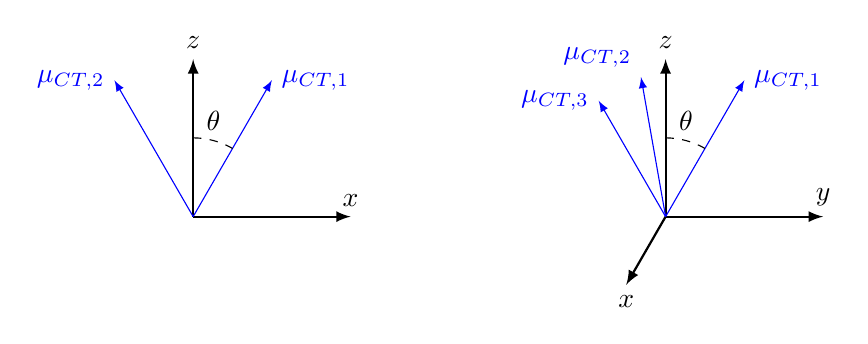
\begin{tikzpicture}
		\begin{scope}
			\draw[-latex,thick] (0,0) -- +(0,2) node[above]{$z$};
			\draw[-latex,thick] (0,0) -- +(2,0) node[above]{$x$};
			\draw[-latex,blue] (0,0) -- (60:2) node[right]{$\mu_{CT,1}$};
			\draw[dashed] (0,1) arc(90:60:1) node[midway,above]{$\theta$};
			\draw[-latex,blue] (0,0) -- (120:2) node[left]{$\mu_{CT,2}$};
		\end{scope}
		\begin{scope}[xshift=6cm]
			\draw[-latex,thick] (0,0) -- +(0,2) node[above]{$z$};
			\draw[-latex,thick] (0,0) -- +(2,0) node[above]{$y$};
			\draw[-latex,thick] (0,0) -- +(-120:1) node[below]{$x$};
			\draw[-latex,blue] (0,0) -- (60:2) node[right]{$\mu_{CT,1}$};
			\draw[dashed] (0,1) arc(90:60:1) node[midway, above]{$\theta$};
			\draw[-latex,blue] (0,0) -- (100:1.8) node[anchor=south east]{$\mu_{CT,2}$};
			\draw[-latex,blue] (0,0) -- (120:1.7) node[left]{$\mu_{CT,3}$};
		\end{scope}
	\end{tikzpicture}
	\caption{Representation of the $\theta$-dependent charge-transfer dipoles ($\mu_{CT}$) in the 3-state (left) and 4-state (right) models.}
	\label{sc:mu}
\end{scheme}

\paragraph{Four-state $C_{3v}$ system.}  
This model consists of three charge transfer (CT) states arranged at \SI{120}{\degree} intervals in the $xy$-plane, with the first dipole aligned along the $y$-axis. Additionally, each dipole forms an angle $\theta \in [0, \nicefrac{\pi}{2}]$ with the $z$-axis, as illustrated in Scheme~\ref{sc:mu}. The dipole moments are therefore given by:  
\begin{equation*}
	\vec{\mu}_{CT,1} = \mu_{CT} \begin{pmatrix} 0 \\ \sin\theta \\ \cos\theta \end{pmatrix},  
	\quad  
	\vec{\mu}_{CT,2,3} = \frac{\mu_{CT}}{2} \begin{pmatrix} \pm\sqrt{3}\,\sin\theta \\ -\sin\theta \\ 2\,\cos\theta \end{pmatrix}.
\end{equation*}
In the limit  $\theta \to \nicefrac{\pi}{ 2}$, this model reduces to a $D_{3h}$ system.

\paragraph{Five-state $T_d$ system.}  
For completeness, the $T_d$ geometry is also considered \cite{choNonlinearOpticalProperties2002}. In this contribution, the corresponding CT dipole moments are (arbitrarily) defined as:  
\begin{align*}
	\vec{\mu}_{CT,1} &= \mu_{CT} \frac{\sqrt{3}}{3} \begin{pmatrix} 1 \\ 1 \\ 1 \end{pmatrix},  
	\quad  
	\vec{\mu}_{CT,2} = \mu_{CT} \frac{\sqrt{3}}{3} \begin{pmatrix} 1 \\ -1 \\ -1 \end{pmatrix}, 
	\quad
	 \vec{\mu}_{CT,3} = \mu_{CT} \frac{\sqrt{3}}{3} \begin{pmatrix} -1 \\ -1 \\ 1 \end{pmatrix},  \\
	\vec{\mu}_{CT,4} &= \mu_{CT} \frac{\sqrt{3}}{3} \begin{pmatrix} -1 \\ 1 \\ -1 \end{pmatrix}.
\end{align*}

\section{Results}

\subsection{Individual components}

In this first part, a tensor component is assumed to follow the form:
\begin{equation*}
	\tilde \beta_{\zeta\eta\kappa} \propto M(m_{CT}) \times E(m_{CT},t,T) \times \Theta(\theta),
\end{equation*}
with the corresponding decomposition summarized in Table~\ref{tab:dec} (the full expressions are provided in the SI).
Certain components exhibit very similar expressions across different systems, leading to comparable $m_{CT}$ dependencies. This is the case for $\beta_{zzz}$ in the VB-$n$CT models for $n\in[1,3]$, as well as $\beta_{yyy}$ and $\beta_{(xyz)}$ for the VB-3CT and VB-4CT models, respectively. 

\begin{table}
	\centering
	\begin{tabular}{llll}
		\toprule
		&$M(m_{CT})$ & $E(m_{CT}, t, T)$ & $\Theta(\theta)$ \\
		\midrule
		\multicolumn{4}{c}{2-state $C_{\infty v}$} \\
		\midrule
		$\tilde\beta_{zzz}$ & $-m_{CT}\,(1-m_{CT}^2)$ & $\Delta E_{0f}^{-2}$ & \\
		\midrule
		\multicolumn{4}{c}{3-state $C_{2v}\rightarrow D_{\infty h}$}\\
		\midrule
		$\tilde\beta_{zzz}$ & $-m_{CT}\,(1-m_{CT}^2)$ & $\Delta E_{0f}^{-2}$ & $\cos^3\theta$ \\
		$\tilde\beta_{(zxx)}$ & $(1-m_{CT}^2)$ & $2\,\Delta E_{0f}^{-1}\Delta E_{0e}^{-1}+\Delta E_{0e}^{-2}$ & $\sin^2\theta\cos\theta$\\
		\midrule
		\multicolumn{4}{c}{4-state $C_{3v}\rightarrow D_{3h}$} \\
		\midrule
		$\tilde\beta_{zzz}$ & $-m_{CT}\,(1-m_{CT}^2)$ & $\Delta E_{0f}^{-2}$ & $\cos^3\theta$\\
		$\tilde\beta_{(zyy)}$ & $(1-m_{CT}^2)$ & $2\,\Delta E_{0f}^{-1}\Delta E_{0e}^{-1}+\Delta E_{0e}^{-2}$ & $\sin^2\theta\cos\theta$\\
		$\tilde\beta_{yyy}$ & $ (1+m_{CT})$ & $\Delta E_{0e}^{-2}$ & $\sin^3\theta$\\
		\midrule
		\multicolumn{4}{c}{5-states $T_d$} \\
		\midrule
		$\tilde\beta_{(xyz)}$ & $ (1+m_{CT})$ & $\Delta E_{0e}^{-2}$ & \\
		\bottomrule
	\end{tabular}
	\caption{Decomposition of the non-zero components into the functions that describe their behavior,  for the different VB-$n$CT models ($n\in[1,4]$).}
	\label{tab:dec}
\end{table}

\clearpage

\subsection{Evolution of the response with the symmetry}

Then, the evolution of the different invariants with the symmetry of the system are broadly addressed.
The evolution of $\tilde\beta_{SHS}$ is shown in Fig.~\ref{fig:beta}. To present the various results in a single graph, the values are plotted along a pathway illustrated in Scheme~\ref{sc:symmetry}. This pathway represents a continuous transformation, starting from the VB-CT model and gradually adjusting the $\mu_{CT}$ values and $\theta$ angle to transition to the VB-4CT model.

\begin{figure}[!h]
	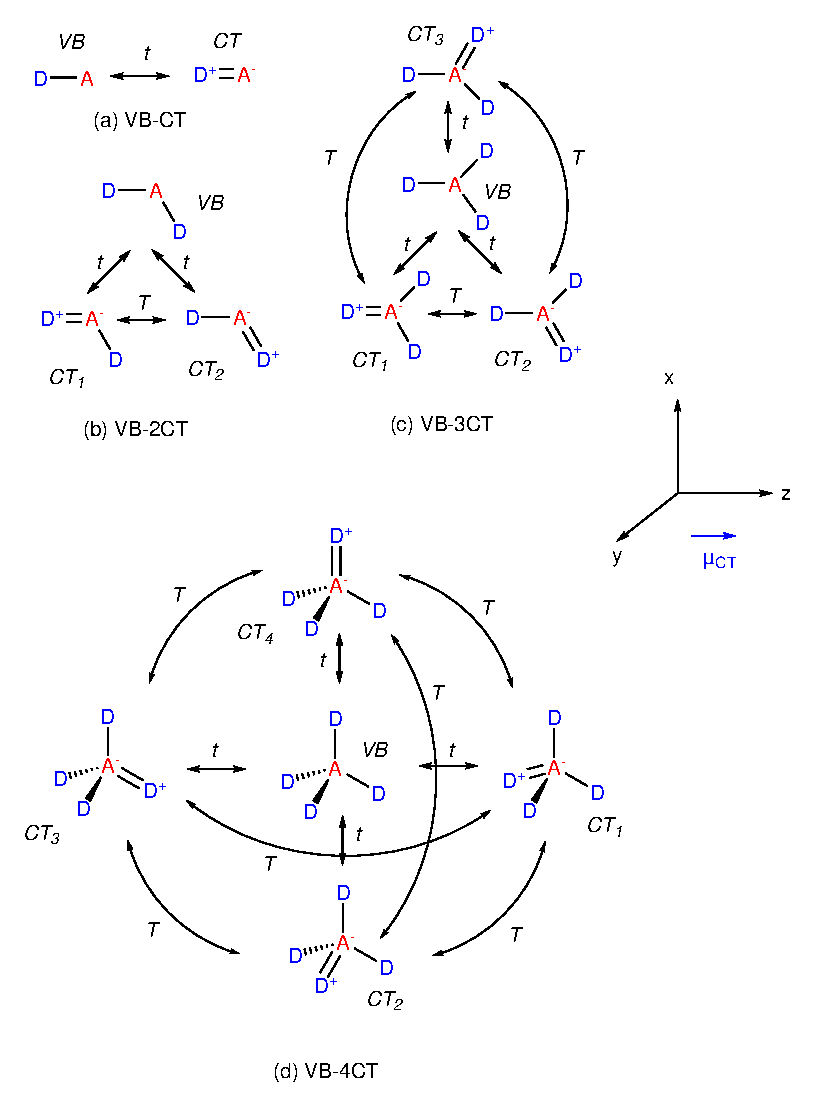
\includegraphics[width=.8\linewidth]{Figure2}
	\caption{Evolution of $\tilde \beta_{SHS}$ (top, unitless) and $DR_{SHS}$ (bottom) as a function of the symmetry of the system and the charge transfer character of the ground state ($m_{CT}$), with $T=t/2$.}
	\label{fig:beta}
\end{figure}

\begin{scheme}
	\centering
	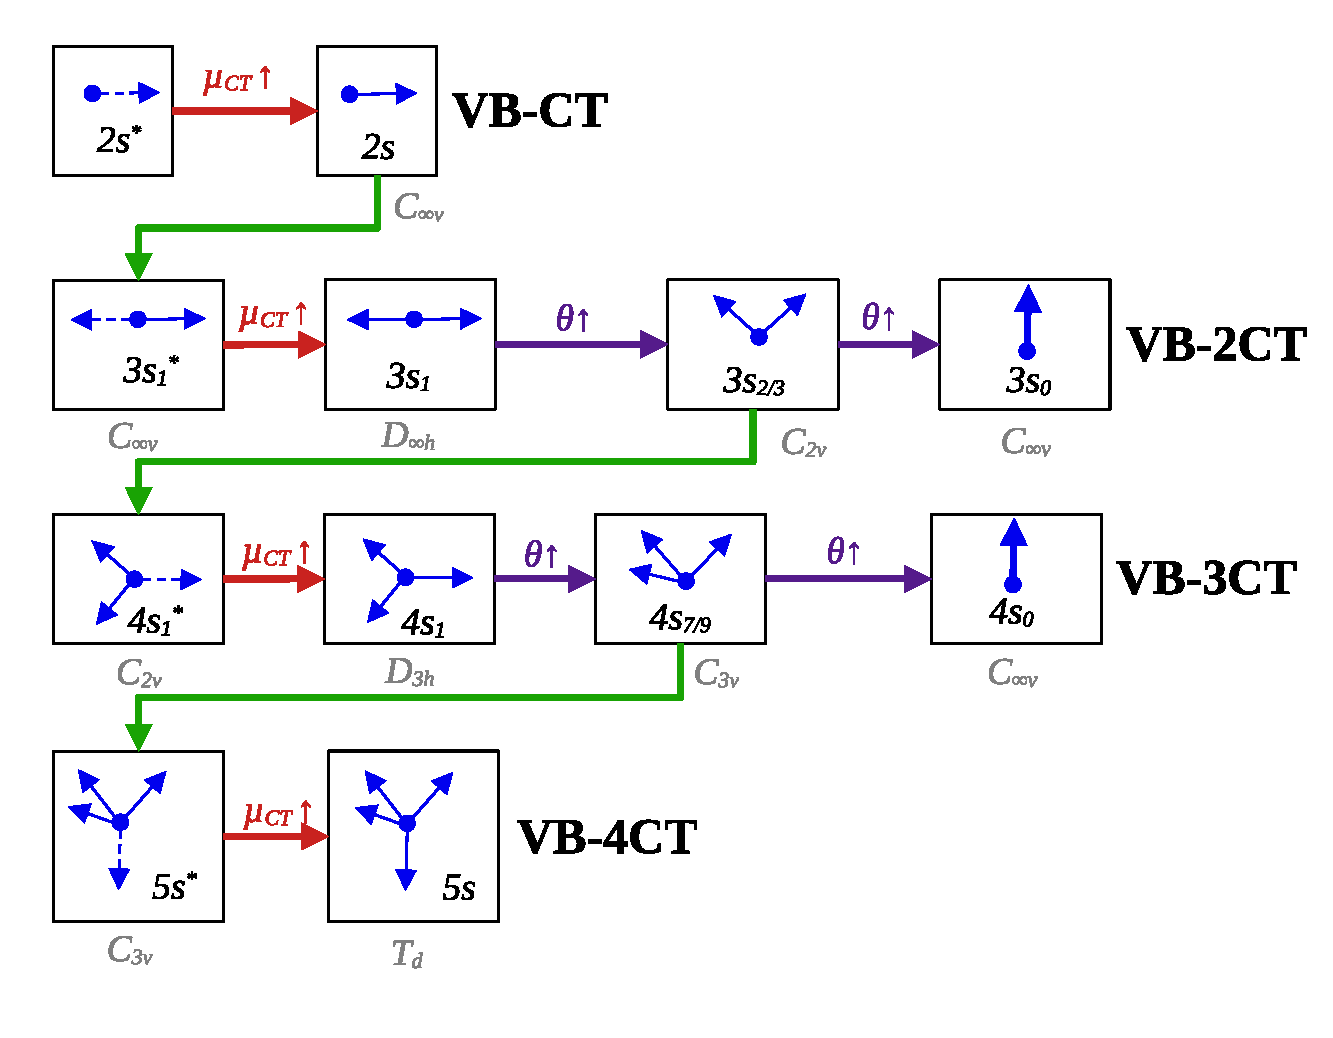
\includegraphics[width=.8\linewidth]{Scheme4}
	\caption{Set of transformations for the 2-state to 5-state systems explored in this article. The notation ``$ks$" ($k \in [2,5]$) represents a $k$-state system, corresponding to a VB-$(k-1)$CT model (the CT dipoles, $\vec\mu_{CT}$, are indicated by blue arrows). The notation "$ks^\star$" refers to a $k$-state model in which one of its $\vec\mu_{CT} = \vec 0$ (indicated by a dashed line).  Additionally, ``$ks_x$" ($k=3,4$ and $x \in [0,1]$) denotes a 3- or 4-state model with $\theta = \frac{x\pi}{2}$. Thus, a $ks^\star \to ks$ symmetry transition corresponds to an increase in the initially missing $\mu_{CT}$, leading to higher symmetry. Meanwhile, a $ks_1 \to ks_0$ transition corresponds to a decrease in $\theta$, ultimately resulting in a $C_{\infty v}$ symmetry where all CT dipoles are parallel.}
	\label{sc:symmetry}
\end{scheme}


Looking at Fig.~\ref{fig:beta}, four main trends can be identified: \begin{inparaenum}[(i)]
	\item systems with non-equivalent $\mu_{CT}$'s display smaller $\tilde\beta_{SHS}$ than their fully-equivalent counterparts,
	\item large values of $m_{CT}$ are required to achieve high $\tilde\beta_{SHS}$,
	\item highly symmetric systems ($D_{3h}$ and $T_d$) exhibit the largest $\tilde\beta_{SHS}$ values, and
	\item due to symmetry constraints, the values for $C_{2v}$ at large $\theta$ and $D_{\infty h}$ are close to or exactly zero.
\end{inparaenum}
Specifically, for $m_{CT} = 0.75$, the following ordering of responses is observed:
\begin{align}
	D_{3h} > C_{3v}\,(\text{large } \theta) > T_d > C_{2v}\,(\text{moderate } \theta) > C_{\infty v} \sim C_{2v}\,(\text{small } \theta) \sim C_{3v}\,(\text{small } \theta). \label{eq:ordering}
\end{align}
This trend persists at lower $m_{CT}$ values, albeit with reduced values and differences between the symmetries. For $m_{CT} < -0.5$, the $\tilde\beta_{SHS}$ values tend to converge and become nearly indistinguishable across symmetries.

A decomposition into the dipolar and octupolar components (Fig.~\ref{fig:betaJ}) provides further insight. On the one hand, large $\tilde\beta_{SHS}$ values are generally associated with dominant octupolar contributions (whose curves almost mirror the $\tilde\beta_{SHS}$ evolution), consistent with the findings of Zyss\cite{zyssMolecularEngineeringImplications1993}. Such systems also exhibit low depolarization ratios (DR$_{SHS}$), approaching the octupolar limit of $\nicefrac{3}{2}$. On the other hand, systems with strong dipolar character, namely $C_{\infty v}$ and $C_{2v}$ symmetries which correspond to the VB-CT and VB-2CT models, display significant $\tilde\beta_{SHS}$ values at moderate $m_{CT}$. This behavior is well-known in the context of the VB-CT model\cite{barzoukasTwostateDescriptionHyper1996}, which reaches a maximum response at $m_{CT} = \pm\frac{\sqrt{5}}{5}$.

\begin{figure}[!h]
\includegraphics[width=.8\linewidth]{Figure3}
\caption{Evolution of the reduced rotational invariants of the first hyperpolarizability tensor ($|\tilde \beta_{J=1}|^2$ and $|\tilde \beta_{J=3}|$, both unitless) as a function of the symmetry of the system and the charge transfer character of the ground state ($m_{CT}$), with $T=t/2$.}
\label{fig:betaJ}
\end{figure}

The behavior of the VB-2CT model is more complex to interpret, as it also depends on the angle $\theta$. Two representative examples are shown in Fig.~\ref{fig:3sttheta}, which illustrate that the maximum of $\tilde\beta_{SHS}$ occurs at positive $m_{CT}$ values and around $\theta \approx \SI{54.9}{\degree}$. This angle closely matches the maximum of the function $\sin^2\theta\cos\theta$, which is located at $\theta = \tan^{-1}(\sqrt{2}) \approx \SI{54.72}{\degree}$. This observation suggests that, among the two nonzero and independent tensor components in this model [$\beta_{zzz}$ and $\beta_{(zxx)} $, Table \ref{tab:dec}], $\beta_{(zxx)} \propto \sin^2\theta\cos\theta / (\Delta E_{ge}\,\Delta E_{gf})$ is the dominant one in this region.  This is in agreement with the observation of Yang and its co-worker\cite{yangLargeOffDiagonalContribution2003} for these systems.
The influence of the parameter $T$ is also evident: smaller values of $T$ yield larger $\tilde\beta_{SHS}$ amplitudes, with the peak shifting to higher $m_{CT}$ values. This behavior is consistent with the inverse of the transition energies, since $\Delta E_{0e}^{-1}\,\Delta E_{0f}^{-1} \propto T^{-1}$. This evolution will be further investigated below.


\begin{figure}[!h]
	\includegraphics[width=.7\linewidth]{Figure4a}
	\includegraphics[width=.7\linewidth]{Figure4b}
	\caption{Evolution of $\tilde\beta_{SHS}$  of the VB-2CT with $m_{CT}$ and $\theta$, with $T=t/2$ (top) and $T=t/10$ (bottom). Dashed line gives the approximate position of the maximum, found by taking the maxima in each heatmap.}
	\label{fig:3sttheta}
\end{figure}

\clearpage
\subsection{Further investigations on the systems with a large response}

As seen in the previous section, the systems exhibiting the largest responses are the VB-3CT and VB-4CT models, particularly at $m_{CT} \to 1$ and $\theta \to \SI{90}{\degree}$ (corresponding to high symmetries). The corresponding approximate expressions for $\tilde\beta_{SHS}$ near $m_{CT} = 1$ are (notice that absolute values are used):\begin{align}
	&\tilde\beta_{SHS}[D_{3h}, m_{CT}=1] = \frac{\sqrt{42}}{63\xi^2}\,\left|1-\dfrac{2\,\sqrt{\frac{3}{2}\,(1-m_{CT})}}{3T}\right|, \text{ and}\label{eq:highsym4}\\ &\tilde\beta_{SHS}[T_d, m_{CT}=1]  = \frac{\sqrt{21}}{84\xi^2}\,\left|1-\dfrac{\sqrt{\frac{1}{2}\,(1-m_{CT})}}{T}\right|,\label{eq:highsym5}
\end{align}
which both display a depolarization ratio of $\frac{3}{2}$.
Although these approximations quickly underestimate the values for $m_{CT} < 1$ (see Fig.~\ref{fig:series}), they confirm that the invariants reach their maxima at $m_{CT} = 1$, help rationalize the ordering established in Eq.~\eqref{eq:ordering}, and provide upper bounds for these systems. 
Moreover, these results indicate that achieving large responses requires minimizing $T$ (and, to some extent, $t$).

\begin{figure}[!h]
	\includegraphics[width=.6\linewidth]{Figure5}
	\caption{Evolution of $\tilde\beta_{SHS}$ for high-symmetry systems for $m_{CT}\to 1$, with $T=t/2$. Dashed line is an approximation obtained with a series around $m_{CT}=1$ [Eqs.~\eqref{eq:highsym4}-\eqref{eq:highsym5}].}
	\label{fig:series}
\end{figure}

\clearpage

To extend this analysis to the $C_{3v}$ systems, one can examine the individual tensor components (reported in the SI) near $\theta = \SI{90}{\degree}$, setting $m_{CT} = 1$. From Table \ref{tab:dec},the only nonzero components is $\beta_{yyy} = -\beta_{(yxx)} \propto \sin^3\theta$, as illustrated in Fig.~\ref{fig:theta}, where the approximate expressions from Eq.~\eqref{eq:highsym4}, multiplied by the corresponding sine dependencies gives the $\theta$ evolution. This confirms that for this system, $\theta=\SI{90}{\degree}$ result in an extrema.

\begin{figure}[!h]
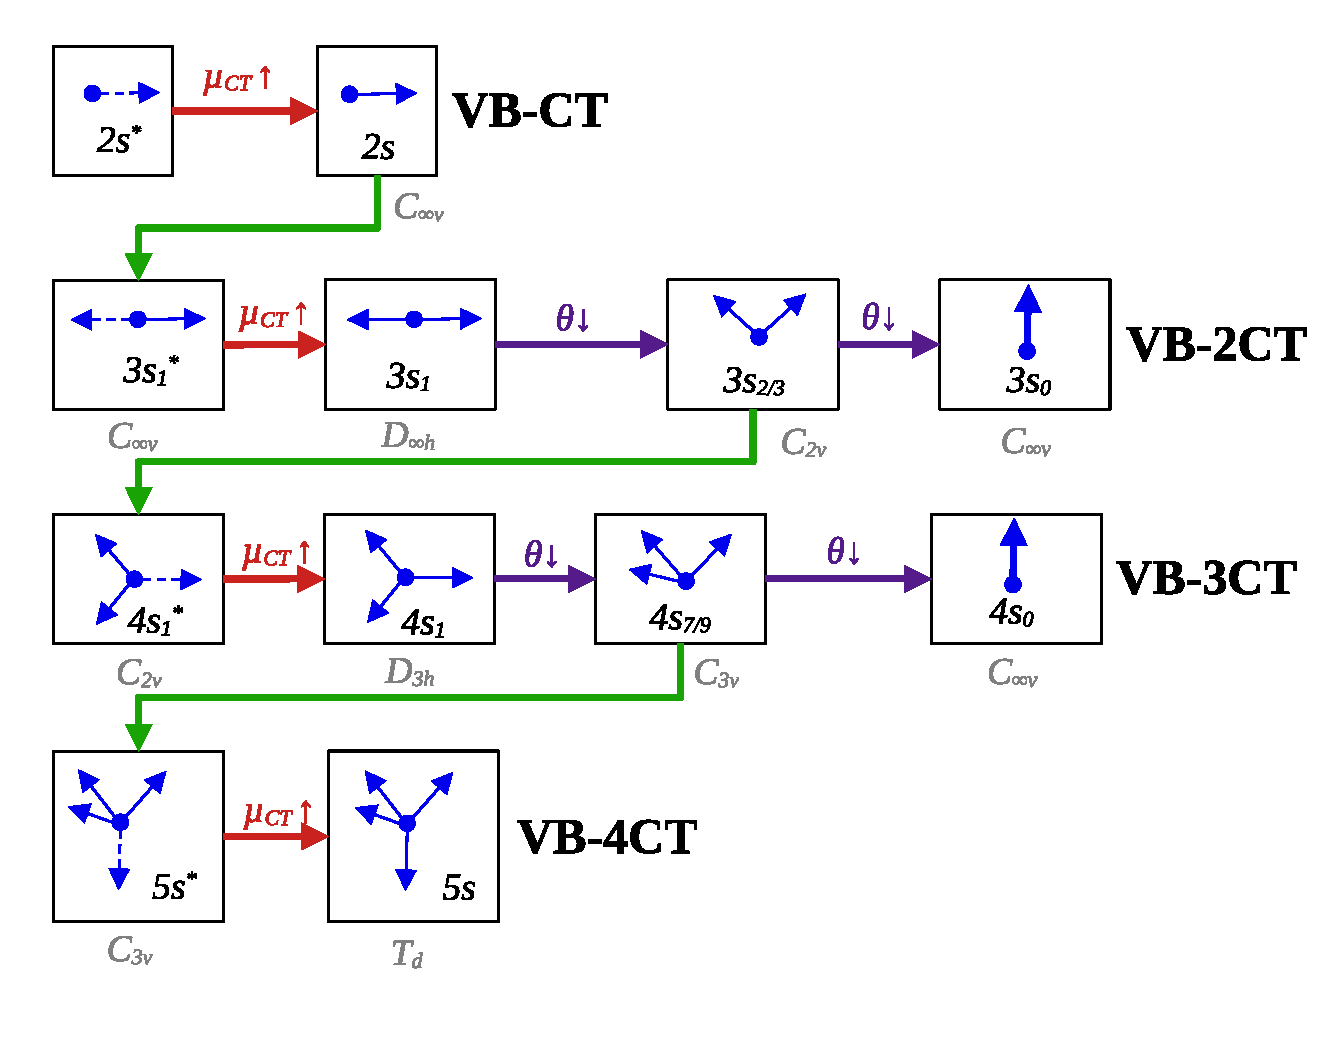
\includegraphics[width=.6\linewidth]{Figure6}
\caption{Evolution of $\tilde\beta_{SHS}$ of  the VB-3CT model with $\theta$ at $m_{CT}= 1$, with $T=t/2$.}
\label{fig:theta}
\end{figure}

Then, and since the seminal work of Oudar and Chemla\cite{oudarHyperpolarizabilitiesNitroanilinesTheir1977} on the first hyperpolarizability, the VB-CT model has been instrumental in elucidating the structure–NLO activity relationship in materials\cite{luValenceBondChargeTransferModel1994,barzoukasTwostateDescriptionHyper1996,barzoukasTWOFORMDESCRIPTIONPUSHPULL1996,blanchard-desceTwoformTwostateAnalysis1998a}. As previously mentioned, the extrema are located at $m_{CT} = \pm\frac{\sqrt{5}}{5}$. Accordingly, the values of $\tilde\beta_{SHS}$ at these maxima are:
\begin{align}
	\tilde\beta_{SHS}[C_{\infty v}, m_{CT}=\pm\nicefrac{\sqrt{5}}{5}] = \frac{6\sqrt{42}}{875} \label{eq:2stmax}
\end{align}
It is associated with DR$_{SHS}=5$ which constitute in both cases the so-called 1D limit.

Summarizing the observations so far, one gets, for a given value of $\xi=\nicefrac{T}{t}$, the following relationships :
\begin{align}
	\tilde\beta_{SHS}[C_{3v}, m_{CT}=1]  &= \underbrace{\frac{4\sqrt{2}}{3}}_{\approx 1.89}\sin^3(\theta)\,\tilde\beta_{SHS}[T_d, m_{CT}=1]\nonumber \\
	&=  \underbrace{\frac{125}{54 \xi^2}}_{\approx 2.32 / \xi^2}\sin^3(\theta)\,\tilde\beta_{SHS}[C_{\infty v}, m_{CT}=\pm\nicefrac{\sqrt{5}}{5}].
\end{align}
This is one of the main result of this paper, which links the theoretical upper bonds for SHS first hyperpolarizability invariants of different symmetries.

Finally, although it is not possible to derive an analytical expression for the maximum of $\beta_{SHS}$ in the VB-2CT model\cite{yangLargeOffDiagonalContribution2003}, it can be investigated numerically (Fig.~\ref{fig:3stmax}). The results indicate that for small values of $\xi = T/t$, $\beta_{SHS}$ reaches a maximum near $m_{CT} \approx 1$ and $\theta \approx \SI{54.7}{\degree}$, which corresponds to DR$_{SHS}=\nicefrac{27}{11}\approx 2.45$. This situation, when $m_{CT} > 0$, corresponds to a regime where $\beta_{(zxx)}$ dominates, particularly through its $\Delta E_{ge}^{-2}$ contribution (Table \ref{tab:dec}). It should be noted that $m_{CT}$ cannot exactly equal 1, as this would result in $\beta_{zzz} = \beta_{(zxx)} = 0$. Consequently, achieving large $\beta_{SHS}$ values requires a delicate balance between maximizing $m_{CT}$ and minimizing $T$. This numerical analysis nevertheless suggests that the values are, for ideal $\theta$ and $m_{CT}$ values, larger than the maximum predicted for the $C_{\infty v}$ (VB-CT) symmetry [from Eq.~\eqref{eq:2stmax}, $\tilde\beta_{SHS}=0.04$], and that the upper bound for $\tilde\beta_{SHS}$ is approximately 0.225 for $m_{CT}\in(0.97,0.98]\land \theta = \tan^{-1}(\sqrt{2}) \land \xi \leq \num{e3}$. However, in this case, the predicted first hyperpolarizability responses for the $C_{3v}$ (VB-3CT) and $T_d$  (VB-4CT) symmetries are orders of magnitude larger.

\begin{figure}
	\centering
	\includegraphics[width=.49\linewidth]{Figure7}
	\caption{Evolution of $\tilde\beta_{SHS}$ (top) and of its maximum (found numerically, blue curve in the top and middle panels), with $\xi = T/t$, for the VB-2CT model, and of the position of this maximum (bottom).}
	\label{fig:3stmax}
\end{figure}


\clearpage
\section{Further discussions, conclusions, and outlooks}

In this paper, VB-$n$CT models ($n \in [1,4]$) were investigated to assess the influence of symmetry and electronic structure parameters, particularly the ground-state charge-transfer character (quantified by the VB-CT mixing parameter $m_{CT}$), on the NLO response. Special attention was given to quantities accessible via second and third harmonic scattering techniques, namely $\beta_{SHS}$ and its corresponding depolarization ratio.

The results confirm that, in agreement with previous studies, a large $m_{CT}$ value combined with a small $T$ integral yields the largest responses. In particular, symmetry considerations favor the $C_{3v}$ symmetry (VB-3CT), especially at $\theta = \SI{90}{\degree}$, where it corresponds to a $D_{3h}$ symmetry, followed by the $T_d$ case. Other cases were explored, but they lead to less important $\beta_{SHS}$ values.
In all scenarios, ensuring a large $\mu_{CT}$ value and achieving a small ratio $\xi = T/t$ is critical for maximizing the NLO response, which, in practical terms, requires minimizing the first excitation energy $\Delta E_{ge}$.\textcolor{red}{(... and end up with a quasi-degenerated case?)}

While feasible in principle, the different parameters ($t$, $T$, $m_{CT}$, $\mu_{CT}$) are generally difficult to extract directly from experimental measurements. Among them, $\mu_{CT}$ can be inferred from UV/Vis absorption spectra, but the others are less accessible. As a result, theoretical calculations are of primary importance for the design of new compounds with enhanced NLO responses.
For instance, estimating $t$ or $T$ can be achieved through projection methods, which involve partitioning the electronic Hamiltonian. A recent application of such approaches to intramolecular donor-acceptor systems can be found in the work of Gillet \emph{et al.} \cite{gilletElectronicCouplingCalculations2016}, following the methodology introduced by Baumeier \emph{et al.} \cite{baumeierDensityfunctionalBasedDetermination2010}. More empirical models are also widely used: for example, the electron-in-a-box model, with its characteristic $\Delta E \propto L^{-2}$ dependence (where $L$ is the box size), predicts that increasing the length of a $\pi$-conjugated pathway (a common strategy to enhance NLO responses) leads to a decrease in $t$, up to a given point\cite{luValenceBondChargeTransferModel1994}.
More generally, both $t$ and $T$ are dominated by electrostatic interactions at large intermolecular separations and therefore decrease with distance. For $T$ in particular, Förster theory can be used to approximate interactions between CT states via dipole-dipole coupling, leading to $T \propto r^{-3}$, where $r$ is the distance between dipoles \cite{sistoInitioNonadiabaticDynamics2014}.
Finally, $m_{CT}$ (or equivalently $\ell_{CT}$) has been linked to structural parameters such as the bond length alternation (BLA), as reported by Barzoukas \emph{et al.} \cite{barzoukasTWOFORMDESCRIPTIONPUSHPULL1996,barzoukasTwostateDescriptionHyper1996}, with a similarly strong correlation observed with the bond order alternation (BOA) \cite{dellaiDynamicEffectsNonlinear2024}.

In practice, achieving the ideal conditions explored in this study remains a significant challenge. One major difficulty is that real compounds are rarely perfectly symmetric and often possess multiple CT excited states of importance\cite{zhangTheoreticalInvestigationFirst2013}, both of which can impact their NLO responses. Furthermore, obtaining large $m_{CT}$ values requires a delicate balance between donor and acceptor strengths \cite{beaujeanUnravelingSymmetryEffects2022,postilsSecondorderNonlinearOptical2024}, which is not easily achieved synthetically.
While VB-CT models associated with quasi-one-dimensional compounds have been highly successful \cite{bourhillExperimentalDemonstrationDependence1994,daltonOrganicElectroOpticsPhotonics2015,wuHighperformanceOrganicSecond2020} and continue to drive the field forward \cite{dalton25YearsOrganic2019,dubuisNonlinearOpticalResponses2023,dellaiDynamicEffectsNonlinear2024}, octupolar systems are still comparatively less common, although the present work reaffirms their relevance. Hopefully, since the seminal contributions of Zyss \cite{zyssMolecularEngineeringImplications1993}, a wide range of carbon-based architectures have been explored, including $C_{2v}$-like \cite{yangLargeOffDiagonalContribution2003,castetSecondorderNonlinearOptical2021,postilsSecondorderNonlinearOptical2024} and octupolar systems \cite{choElementaryDescriptionNonlinear1998,panjaSumoverstateSchemeAnalysis2010,beaujeanMultiStateSecondOrderNonlinear2022}, offering numerous powerful design strategies.
Beyond purely organic molecules, organometallic compounds present another powerful avenue, leveraging a variety of low-energy charge-transfer processes, such as metal-to-ligand charge transfer (MLCT). Among these, ruthenium- and iron-based complexes have been the most extensively studied \cite{coeDevelopingIronRuthenium2013,ashcroftMolecularEngineeringOrganic2019}, though other metals have also been successfully incorporated into NLO-active materials \cite{costesSynthesisCrystalStructures2005,lamereSynthesisCharacterizationNonlinear2006,lacroixSecondorderNonlinearOptics2016}. Here, different ligands coordinated to the metal center enable fine-tuning of the electronic properties and facilitate access to a wide range of molecular symmetries \cite{ashcroftMolecularEngineeringOrganic2019,beaujeanUnravelingSymmetryEffects2022,hoodSynthesisOpticalNonlinear2024}. Metal-organic frameworks (MOFs) also fall within this class of materials and, when carefully designed, can exhibit remarkable NLO properties \cite{medishettyNonlinearOpticalProperties2017,chengNonlinearOpticalProperties2021}.



\begin{acknowledgement}
	This work was supported by the Excellence of Science (EOS) programme  ECOBAT (EOS No. 40007515). 
\end{acknowledgement}

\begin{suppinfo}
	For each VB-$n$CT model ($n\in[1,4]$): \begin{inparaenum}[i)]
		\item the expression for all transition and excited state dipole moments,
		\item the corresponding expression for all non-null tensor components, and
		\item the expression of the tensor invariants.
	\end{inparaenum}
\end{suppinfo}


\bibliography{biblio}
\end{document}
